\documentclass[xcolor=pdftex,dvipsnames,table,aspectratio=169]{beamer}
%\documentclass[xcolor=pdftex,dvipsnames,table,handout,aspectratio=169]{beamer}

%\setbeameroption{show notes}

\usepackage{bm,graphicx,multirow,amsmath,tikz} %fancybox,
\usepackage{color}%,textpos}
\usepackage[round]{natbib}
\usepackage[normalem]{ulem}
\usepackage{hyperref}
\usepackage{lastpage}
\usepackage{array}
\usepackage{color}
\usepackage{framed}
\usepackage{hyperref}

% Define Western colours
\definecolor{western}{rgb}{.306,.152,.524}
\definecolor{westerngray}{rgb}{.512,.508,.524}

%% Define BEAMER colours
\setbeamercolor{frametitle}{bg=western,fg=white}
\setbeamercolor{framesubtitle}{bg=western,fg=black}
\setbeamercolor{title}{fg=white,bg=western}
\setbeamercolor{author}{fg=white,bg=western}
\setbeamercolor{institute}{fg=white,bg=western}
\setbeamercolor{date}{fg=white,bg=western}

%% Set BEAMER fonts
\setbeamerfont{title}{shape=\bf}
\setbeamerfont{frametitle}{shape=\sc,size=\Large}
\setbeamerfont{framesubtitle}{shape=\sc,size=\Large}
\setbeamerfont{footline}{shape=\sc}

%% Define BEAMER toc
\setbeamercolor{section in toc}{fg=western}
\setbeamercolor{subsection in toc}{fg=westerngray}
\setbeamertemplate{sections/subsections in toc}[ball]

%% Define BEAMER background
\setbeamercolor{background canvas}{bg=white}

%% Define BEAMER footer
\setbeamertemplate{navigation symbols}{}
\setbeamercolor{footline}{fg=white,bg=western}
\setbeamertemplate{footline}{%
  \begin{beamercolorbox}[wd=\paperwidth]{footline}
    \vskip5pt

    \raisebox{.05in}{
      \scriptsize{\bf \insertshorttitle}
    }
    \hfill
    \raisebox{.05in}{
      \scriptsize{\bf \insertframenumber/\inserttotalframenumber} 
    }
    \hspace{5pt}

    \vskip5pt
  \end{beamercolorbox}
}

%% Define BLOCK environment
\setbeamercolor{block title}{fg=western}
\setbeamerfont{block title}{series=\bfseries}

%% Define ENUMERATE and ITEMIZE environements
\setbeamertemplate{itemize item}[ball]
\setbeamertemplate{enumerate item}[ball]
\setbeamercolor{item projected}{bg=western}

%% Define BEAMER toc
\setbeamercolor{sections/subsections in toc}{fg=blue!75}
\setbeamertemplate{sections/subsections in toc}[ball]

% %% Define SECTION openings
% \AtBeginSection[]{
%   \begin{frame}{\insertshorttitle}
%     \tableofcontents[currentsection,subsectionstyle=hide/hide/hide]
    
%   \end{frame}
% }

%% Define BEAMER frametitle
\addtobeamertemplate{frametitle}{
   \let\insertframetitle\insertsectionhead}{}
\addtobeamertemplate{frametitle}{
   \let\insertframesubtitle\insertsubsectionhead}{}


\makeatletter
  \CheckCommand*\beamer@checkframetitle{\@ifnextchar\bgroup\beamer@inlineframetitle{}}
  \renewcommand*\beamer@checkframetitle{\global\let\beamer@frametitle\relax\@ifnextchar\bgroup\beamer@inlineframetitle{}}
\makeatother

% Define counters for example and exercise
\newcounter{example}
\newcounter{exercise}

% Define example and exercise commands
\renewcommand{\example}
{\stepcounter{example}Example \lecturenum.\arabic{example}}
\newcommand{\examplectd}
{Example \lecturenum.\arabic{example}\ ctd}
\newcommand{\exercise}
{\stepcounter{exercise}Exercise \lecturenum.\arabic{exercise}}
\newcommand{\exercisectd}
{Exercise \lecturenum.\arabic{exercise}\ ctd}

\newcommand{\lecturenum}{11}

\title[SS2857]{Probability and Statistics I}
\subtitle{\lecturenum. The Hypergeometric and Negative Binomial Distributions}

\date{}

%% Add logo
%% \titlegraphic{\includegraphics[height=2cm]{../uwo_logo_reversed}}

%% Initialize R


\begin{document}

{
\setbeamertemplate{footline}{}
\setbeamercolor{background canvas}{bg=western}

\begin{frame}
  \addtocounter{framenumber}{-1}

  \maketitle
\end{frame}
}

\begin{frame}
  \frametitle{\invisible{Hello}}

  \begin{center}
    \Large{\textbf{3.6 The Hypergeometric and Negative Binomial Distributions}}
  \end{center}

  % \begin{center}
  %   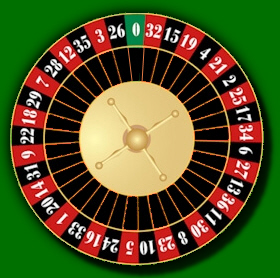
\includegraphics[height=.5\textheight]{roulette_wheel}
  % \end{center}

\end{frame}

\begin{frame}
  \frametitle{\invisible{Hello}}

  \begin{center}
    \Large{\textbf{3.6a The Hypergeometric Distribution}}
  \end{center}

  \begin{center}
    
\includegraphics[height=.5\textheight]{figure/audit}
  \end{center}

\end{frame}

\section{The Hypergeometric Distribution}

\begin{frame}

  \begin{block}{Application}
    The hypergeometric distribution models the number of successes when sampling \textit{without replacement} from a fixed population.

  \end{block}

  \begin{block}{Assumptions}
    \begin{enumerate}
    \item The population consists of a finite number of individuals, $N$.
    \item $M$ individuals can be classified as successes and $N-M$ as failures.
    \item A sample of $n$ individuals is chosen so \textit{without replacement} so that each sample is equally likely.
    \end{enumerate}
  \end{block}

  \bigskip

  Mathematically, we write
  \[
    X \sim \mbox{Hypergeometric}(n,M,N).
  \]
\end{frame}


\begin{frame}
  \begin{block}{PMF and CDF}
    \begin{itemize}
    \item PMF: $h(x;n,M,N)=\frac{\binom{M}{x}{\binom{N-M}{n-x}}}
      {\binom{N}{n}}$

      \hspace{1in} $x=\max(0,n-N+M),\ldots,\min(n,M)$
      
    \item CDF: Requires special functions.
    \end{itemize}
  \end{block}

  %\begin{block}{Moment Generating Function}
  %  Requires special functions.

  \begin{block}{Properties}
    \begin{itemize}
    \item Mean: $E(X)=nM/N$

    \item Variance: $V(X)=\left(\frac{N-n}{N-1}\right)\left(\frac{nM}{N}\right)\left(1-\frac{M}{N}\right)$
      
    %\item Skewness: $\gamma_1 =\frac{(N-2M)(N-1)^\frac{1}{2}(N-2n)}{[nK(N-M)(N-n)]^{\frac{1}{2}}(N-2)}$
    \end{itemize}
  \end{block}
  
  \begin{block}{Calculator}
  \url{https://stattrek.com/online-calculator/hypergeometric}
  \end{block}
\end{frame}

\begin{frame}

  \begin{block}{\example}

    An accountant is conducting a financial audit on a big, multinational company. The company has 200 accounts, of which 20 have errors. 

    \bigskip
    Suppose that the accountant checks 10 randomly selected accounts. Let $Y$ be the number of accounts with errors in her sample.
    \begin{enumerate}[a)]
    \item What is the distribution of $Y$?
    \item What is the probability that $Y=2$?
    \item What are the mean and variance of $Y$?
    \end{enumerate}
  \end{block}
\end{frame}

\begin{frame}
  \begin{block}{Binomial Approximation}
    Let $p=M/N$ be the proportion of successes in the population. Then the mean and variance can be rewritten as
    \begin{itemize}
    \item Mean: $E(X)=np$

    \item Variance: $V(X)=\left(\frac{N-n}{N-1}\right)np\left(1-p\right)$
    \end{itemize}

    \bigskip

    If $N$ is much larger than $n$ ($n/N \leq .05$), then $V(X) \approx np(1-p)$, which is the variance of a binomial distribution. In this case we can approximate the distribution of $X$ as
    \[
      X \overset{\cdot}{\sim} \mbox{Binomial}(n,p).
    \]
    The symbol $\overset{\cdot}{\sim}$ is read as ``approximately distributed as''.
    
    \medskip
    
    Your book suggests that this is appropriate when $n/N \leq .05$.
  \end{block}

\end{frame}

\begin{frame}

  \begin{block}{\example}

    An accountant is conducting a financial audit on a big, multinational company. The company has 200 accounts, of which 20 have errors. 

    \bigskip
    Suppose that the accountant checks 10 randomly selected accounts. Let $Y$ be the number of accounts with errors in her sample.
    \begin{enumerate}[a)]
    \item Is it appropriate to approximate the distribution of $Y$ by a binomial?
    \item What is the approximate distribution of $Y$?
    \item Approximate the probability that $Y=2$.
    \item Approximate the mean and variance of $Y$.
    \end{enumerate}
  \end{block}
\end{frame}

\begin{frame}
  \frametitle{\invisible{Hello}}

  \begin{center}
    \Large{\textbf{3.6b The Negative Binomial Distribution}}
  \end{center}

  \begin{center}
    
\includegraphics[height=.5\textheight]{figure/audit}
  \end{center}


\end{frame}

\section{The Negative Binomial Distribution}

\begin{frame}
  \begin{block}{Application}
    The negative binomial distribution models the number of failures in a binomial experiment if trials are repeated until the $r^{th}$ success.
  \end{block}

  \begin{block}{Assumptions}
    \begin{enumerate}
    \item The experiment consists of independent and identical trials.
    \item Each trial has two outcomes (called success and failure).
    \item The probability of success, $p$, is the same for all trials.
    \item The experiment continues until the $r^{th}$ success occurs.
    \end{enumerate}
  \end{block}

  \bigskip

  Mathematically, we write
  \[
    X \sim \mbox{Negative Binomial}(r,p).
  \]
\end{frame}

\begin{frame}
  \begin{block}{PMF and CDF}
    \begin{itemize}
    \item PMF: $nb(z;r,p)=\binom{z+r-1}{r-1}p^{r}(1-p)^z, \quad z=0,1,2,\ldots$
    \item CDF: requires special functions
    \end{itemize}
  \end{block}

  %\begin{block}{Moment Generating Function}
  %  \[
  %    M_Z(t)=\frac{p^r}{[1-e^t(1-p)]^r}
  %  \]
  %\end{block}

  \begin{block}{Properties}
    \begin{itemize}
    \item Mean: $E(Z)=\frac{r(1-p)}{p}$
      
    \item Variance: $V(Z)=\frac{r(1-p)}{p^2}$
      
    %\item Skewness: $\frac{2-p}{\sqrt{r(1-p)}}$
    \end{itemize}
  \end{block}
  
  
\end{frame}

\begin{frame}

\begin{block}{Calculator}
  \url{https://stattrek.com/online-calculator/negative-binomial}
  
  \medskip
  
  Note that the calculator uses a different parametrization of the negative binomial distribution. It counts the number of trials ($x=z + r$) until the $r^{th}$ success.
  \end{block}
  
\end{frame}

\begin{frame}

  \begin{block}{\example}

    An accountant is conducting a financial audit on a big, multinational company. The company has 200 accounts, of which 20 have errors. 

    \bigskip
    Suppose that the accountant samples accounts \textit{with replacement} until she finds 2 with errors. Let $Z$ denote the number of accounts without errors in her sample.
    \begin{enumerate}[a)]
    \item What is the distribution of $Z$?
    \item What is the probability that $Z=10$?
    \item What are the mean and variance of $Z$?
    \end{enumerate}
  \end{block}
\end{frame}

\section{The Geometric Distribution}

\begin{frame}
  \begin{block}{Application}
    The geometric distribution is the special case of the negative binomial distribution that models the number of failures in a binomial experiment if trials are repeated until the $1^{st}$ success.
  \end{block}

  \begin{block}{Assumptions}
    \begin{enumerate}
    \item The experiment consists of independent and identical trials.
    \item Each trial has two outcomes (called success and failure).
    \item The probability of success, $p$, is the same for all trials.
    \item The experiment continues until the $1^{st}$ success occurs.
    \end{enumerate}
  \end{block}

  \bigskip

  Mathematically, we write
  \[
    X \sim \mbox{Geometric}(p).
  \]
\end{frame}

\begin{frame}
  \begin{block}{PMF and CDF}
    \begin{itemize}
    \item PMF: $nb(z;1,p)=p^{1}(1-p)^z, \quad z=0,1,2,\ldots$
    \item CDF: requires special functions
    \end{itemize}
  \end{block}

  \begin{block}{Properties}
    \begin{itemize}
    \item Mean: $E(Z)=\frac{(1-p)}{p}$
      
    \item Variance: $V(Z)=\frac{(1-p)}{p^2}$
      
    %\item Skewness: $\frac{2-p}{\sqrt{r(1-p)}}$
    \end{itemize}
  \end{block}
\end{frame}

\begin{frame}
\begin{block}{Binomial vs Hypergeometric vs Negative Binomial}

The Binomial, Hypergeometric, and Negative Binomial distributions all apply to experiments with repeated trials in which repeated trials result in one of two outcomes (labelled success and failure). 

\begin{center}
\begin{tabular}{lccc}
& Binomial & Hypergeometric & Neg.~Binomial\\
\hline
\# of Trials & Fixed & Fixed & Random\\
Trials are independent & Yes & No & Yes\\
Prob. of Success & Fixed & Varies & Fixed\\
\end{tabular}
\end{center}

\end{block}
\end{frame}

\begin{frame}

  \begin{center}
    \Large{\textbf{Questions?}}
  \end{center}
\end{frame}

\begin{frame}
  \begin{block}{\exercise}
  Suppose that packages of Smarties each contain 30 smarties and that there is a .25 probability that each Smartie is red. For each of the following problems: i) identify the distribution of the random variable, ii) compute the mean and variance, iii) compute the probability provided.
  
  \begin{enumerate}[a)]
  \item The number of red Smarties in a package and the probability that the package contains more than 10 red Smarties.
  \item The number of red Smarties you pick if you draw 5 Smarties without replacement from a pack containing exactly 8 red Smarties. The probability this number is less than 3.
  \item The number of package you must open until you find a package with no red smarties. The probability you open exactly 5000 boxes until finding one with no red candies. 
  \end{enumerate}
  
  \end{block}
\end{frame}

\end{document}
